%Methodenwahl % Begründung der Auswahl

Industrieroboter können eine Vielzahl von verschiedenen Aufgabengebieten übernehmen. Die Aufgabengebiete reichen hierbei von Bedinungs- über Bearbeitungs- bis hin zu Montageabläufen \cite{noauthor_industrieroboter_2020}. Die Schwierigkeit besteht hierbei zunächst die Anforderungen an den erforderlichen Industrieroboter zu definieren und wenn möglich einzugrenzen. Da die Kommunikation mit und ohne ROS getestet werden soll ist es von Vorteil einen Industrieroboter mit einer bereits vorhandenen ROS-Unterstützung zu verwenden. Zudem ist es erforderlich den Industrieroboter über eine direkte Schnittstelle ansprechen zu können um die gewünschten Abläufe, welche geteacht werden sollen, mit einer direkten Kommunikation ohne Netzwerklatenzen testen und einen Vergleich auf Grund des Zeitverhaltens anstellen zu können. Die Interoperabilität mit Simulationsumgebungen ist auch abzuwägen, da die Tests mithilfe einer Simulationsumgebung ohne Sicherheitsbedenken für die bedienende Person durchgeführt werden können und zudem für Regressionstests der Gestenerkennungssoftware praktikabel ohne einen realen Roboter durchgeführt werden können. Im weiteren Verlauf muss zudem die Entscheidung für einen Tiefensensor durchgeführt werden um eine Gestenerkennung, welche zur Steuerung des Inustrieroboters eingesetzt werden soll, realiseren zu können. Bei der Gestenerkennung steht vor allem die Ergonomie und die Sicherheit der bedienenden Person im Vordergrund. Hierbei muss unter anderem beachtet werden, dass zufällige Gesten nicht als Aktion gewertet werden, da dies ansonsten die Sicherheit der bedienenden Person negativ beinflussen kann. Bei der Programmiersprache und Programmierumgebung ist dabei darauf zu achten, dass diese zu ROS kompatibel ist, da ansonsten erheblicher Mehraufwand bei der Umsetzung entstehen würde.


\section{Industrieroboter}
Ein Industrieroboter ist ein universell einsetzbarer Bewegungsautomat, welcher im industriellen Einsatzgebiet eingesetzt wird. Zu erwähnen ist, dass Industrieroboter zumeist auf ein bestimmtes Problem zugeschnitten sind. Aus diesem Grund werden diese je nach der Positionsgenauigkeit, Tragfähigkeit, Arbeitsbereich, Arbeitsgeschwindigkeit und maximaler Reichweite unterschieden. Die maximale Reichweite ist bei ortsfesten Industrierobotern durch die Armlänge und die Freiheitsgrade begrenzt. Im Gegensatz zu ortsfesten Industrierobotern können bewegliche Industrieroboter sich zusätzlich in der Umgebung bewegen und werden daher durch die Bewegungsvorrichtung begrenzt \cite{noauthor_industrieroboter_2020}.

\begin{figure}[htb]
	\centering
	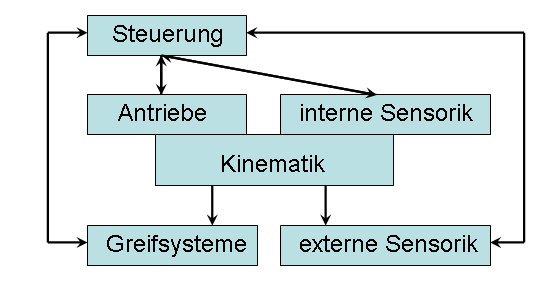
\includegraphics[width=0.6\textwidth]{images/stand_der_technik/Struktur_IR}
	\caption[Struktur eines Industrieroboters]{Struktur eines Industrieroboters \\Quelle: \cite{noauthor_industrieroboter_2020}}
	\label{fig:struktur_eines_industrieroboters}
\end{figure}
\FloatBarrier

Wie in Abbildung \ref{fig:struktur_eines_industrieroboters} zu sehen ist, besteht ein Industrieroboter grundlegend aus einem Roboterarm, welcher auch Manipulator genannt wird, einer Steuerungseinheit, welche für die Überwachungung und Übersetzung der Aktionen auf den spezifischen Industrieroboter zuständig ist und einem Effektor, welcher über ein Greifsystem befestigt wird. Über den Manipulator, welcher Gelenke und Antriebe aufweist, wird die Kinematik realisiert, welche es ermöglicht den Manipulator im Raum zu bewegen. Um jeden Punkt im 3D-Raum ansteuern zu können sind mindestens 3 DOF erforderlich, welche über Gelenke realisiert werden. Um jeden Punkt im Raum mit jeder beliebigen Orientierung ansteuern zu können benötigt es jedoch 6 DOF, wobei 3 Gelenke für translatorische und weitere 3 Gelenke für rotatorische Bewegungsabläufe zuständig sind. Der Effektor kann auf verschiedene Arten realisiert werden. Zumeist ist es jedoch ein Werkzeug, welches z.B. für Schweiß-, Bohr-, Beschichtungs-, Klebe-, Montage- und Schneidearbeiten eingesetzt werden kann. Da der Effektor austauschbar ist, besteht jedoch aber auch die Möglichkeit einen Greifer oder einen anderen spezifisch für eine Aufgabe konzipierten Effektor zu montieren und zu verwenden. Damit die Steuerungseinheit die Gelenkpositionen und Antriebsgeschwindigkeiten ermitteln kann sind zudem Messsysteme erforderlich, welche als interne Sensoren bezeichnet werden. Als optionale Komponente können zudem externe Sensoren beim Industrieroboter verbaut sein, welche unter anderem zur Ermittlung von Objektposition im 3D-Raum und deren Größe verwendet werden können. Je nach Arbeitsumfeld kann es auch erforderlich sein, dass ein System zum Wechseln der Effektoren eingesetzt wird um mehrere Arbeitsschritte mit einem einzigen Industrieroboter durchführen zu können \cite{hagele_aufbau_2006}.

\subsection{Bauformen}
Industrieroboter können entweder zur seriellen oder parallelen Kinematik zugeordnet werden. Der Unterschied besteht darin, dass die Achsen bei der seriellen Kinematik seriell angeordnet sind, wohingegen bei der paralleln Kinematik die Achsen parallel angeordnet werden.

\begin{figure}[htb]
	\centering
	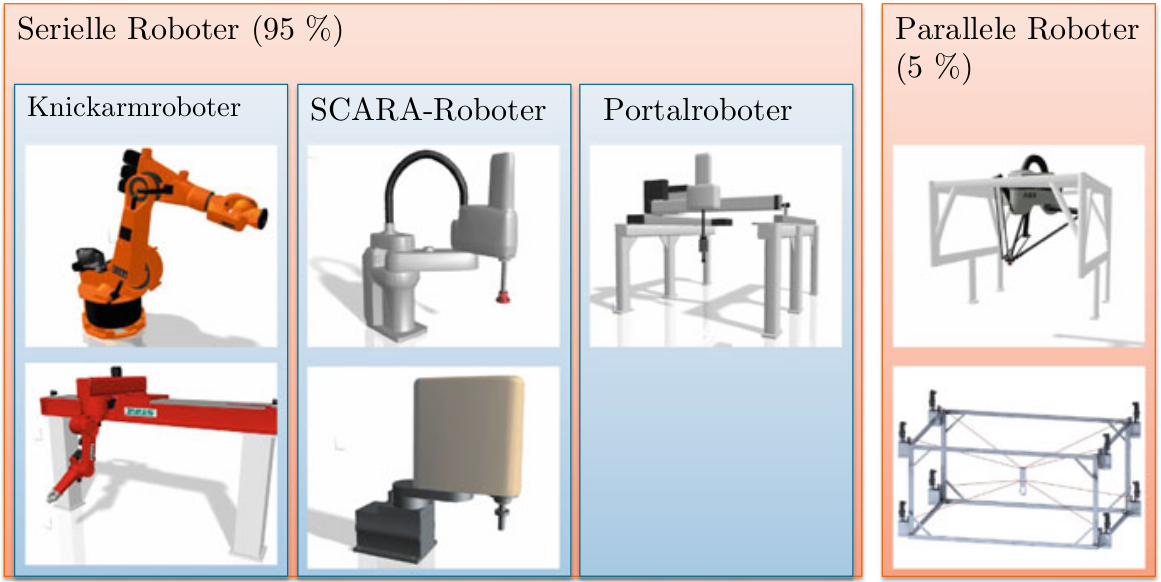
\includegraphics[width=0.9\textwidth]{images/stand_der_technik/bauformen_industrieroboter}
	\caption[Bauformen von Industrierobotern]{Bauformen von Industrierobotern \\Quelle: \cite[18]{pott_industrielle_2019}}
	\label{fig:bauformen_industrieroboter}
\end{figure}
\FloatBarrier

Mit 95\% Anteil haben sich Industieroboter mt serieller Kinematik aufgrund ihrer Bauweise und den bei Knickarmrobotern sehr großen Bewegungsfreiheit durchgesetzt, wie aus der Abbildung \ref{fig:bauformen_industrieroboter} zu entnehmen ist. Nur ein geringer Teil von 5\% der Industrieroboter besitzen eine parallele Kinematik, zu denen unter anderem der Delta- und Seil-Roboter zählen. In der Abbildung \ref{fig:bauformen_industrieroboter} ist der Delta-Roboter im Bereich der parallen Roboter oben und der Seilroboter im unteren Bereich zu sehen. Die parallele Kinematik zeichnet sich dabei durch mindestens eine geschlossene kinematische Kette aus. Zu den seriellen Industrierobotern zählen unter anderem Knick-, SCARA- und Portal-Roboter und alle anderen Roboter, welche eine offene kinematische Kette aufweisen. Industieroboter mit serieller Kinematik zählen zu den am weitest verbreitesten Industrierobotern. Im Gegensatz zu den seriellen Industrierobotern bieten parallele Industrieroboter durch die direkte Verbindung zum Greifsystem den Vorteil, dass die nachfolgenden Glieder und deren Massen nicht wie beim seriellen Industrieroboter die Dynamik des Systems beeinflussen. Dies führt dazu, dass eine sehr hohe Genauigkeit und eine sehr hohe Steifigkeit garantiert werden kann. Zudem sind durch die parallele Kinematik hochpräzise Ansteuerungsmanöver mit sehr hoher Geschwindigkeit durchführbar. Der Nachteil besteht jedoch darin, dass der parallele Industrieroboter ortsfest ist. Die parallele Kinematik zählt daher eher zur Ausnahme und wird aus diesem Grund vermehrt für Pick-and-Place-Aufgaben oder Sondermaschinen eingesetzt, wo Geschwindigkeit, eine hohe Präzision und hohe Dynamik erforderlich ist \cite[17\psqq]{pott_industrielle_2019}.\\

Der Knickarmroboter, welcher zu den seriellen Industrierobotern zählt und zumeist 6 DOF aufweist, bietet den Vorteil, dass dieser für weitere Bewegungsfreiheit auf eine zusätzliche Linearachse montiert werden kann. Dadurch ist es unter anderem Möglich verschiedene Arbeitspositionen eines großen Objekts ansteuern zu können. Da der Knickarmroboter eine armartige Form aufweist, ist dieser zumeist für schwer erreichbare Stellen geeignet. Aufgrund der offenen kinematischen Kette und der Möglichkeit einer sehr großen Nutzlast leidet jedoch die Absolutgenauigkeit darunter. Typischwerweise werden Knickarmroboter für Schweiß-, Handhabungs- und Klebearbeiten eingesetzt. Eine weitere Möglichkeit um serielle Industrieroboter zu realisieren stellen die SCARA-Roboter dar. Diese weisen im Gegensatz zu den Knickarmrobotern weniger Freiheitsgrad. Typischwerweise werden zumeist 3 oder 4 DOF verbaut, wodurch die Bewegungsfreiheit eingeschänkt wird. Zudem sind aufgrund der Bauform nur geringere Arbeitslasten und kleinere Arbeitsbereiche nutzbar. Dies zeigt sich auch beim Aufgabenbereich, welcher großteils in der Montage und Pick-and-Place besteht. Portale, welche auch zu den seriellen Industrierobotern zählen, können sehr hohe Nutzlasten und große Bewegungen durchführen. Sie sind nach den Knickarmrobotern die zweithäufigste Bauform. Zu den Aufgabengebieten zählen Pick-and-Place, Maschinenbestückungen und Kommisionsarbeiten \cite[17\psqq]{pott_industrielle_2019}.

\subsection{Positions- und Bahngenauigkeit}
Die Genauigkeit ist bei Industrierobotern in sehr vielen Aufgabenbereichen, wie z.B Laserschneiden oder Schweißen, sehr entscheident. Eine hohe Genauigkeit spart Kosten und Zeit ein, da eine teure und zeitintensive Nachbearbeitung entfällt. Aus diesem Grund ist es entscheident, dass der Industieroboter für spezielle Aufgabenbereiche eine hohe Positions- und Bahngenauigkeit aufweist. Um die Positions- und Bahngenauigkeit von Industrierobotern beurteilen zu können verwendet man die Absolut- und Wiederholgenauigkeit. Beide Kennwerte beschreiben die Qualität der Übereinstimmung der Realität und des Modells und sind in der ISO 9283, welche die Robotergenauigkeit beinhaltet und beschreibt, standardisiert \cite[28\psqq]{pott_industrielle_2019}.

\begin{figure}[htb]
	\centering
	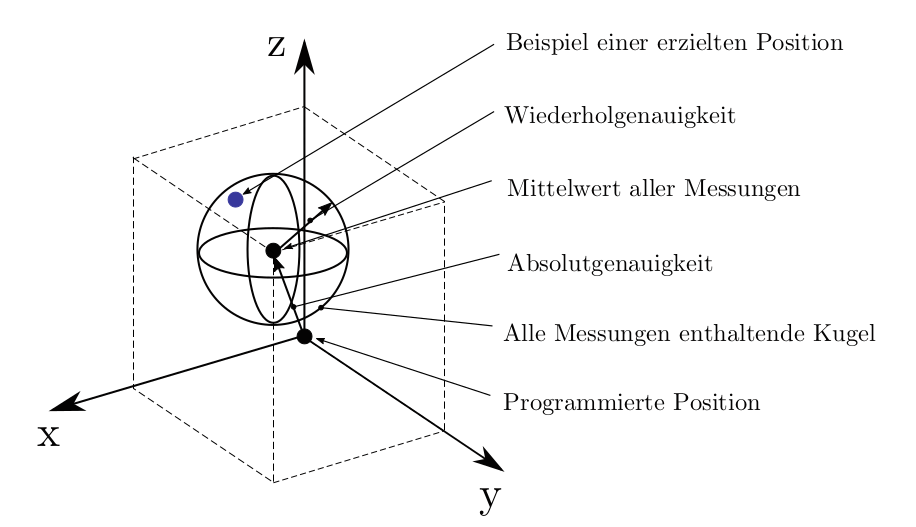
\includegraphics[width=0.78\textwidth]{images/stand_der_technik/absolutgenauigkeit_und_wiederholgenauigkeit}
	\caption[Absolut- und Wiederholgenauigkeit]{Absolut- und Wiederholgenauigkeit \\Quelle: \cite[29]{pott_industrielle_2019}}
	\label{fig:absolutgenauigkeit_und_wiederholgenauigkeit}
\end{figure}
\FloatBarrier

In der Abbildung \ref{fig:absolutgenauigkeit_und_wiederholgenauigkeit} ist der Zusammenhang zwischen der Absolut- und Wiederholgenauigkeit zu erkennen. Die Wiederholgenauigkeit wird ermittelt indem der Industrieroboter über mehrere Zyklen hinweg immer wieder die gleiche Pose anfährt. Hierbei beeinflussen systematische Gegebenheiten, wie z.B. termische Ausdehnung durch Umgebungstemperatur, sowie aber auch durch die Motorwärme, Justagefehler der Achsen oder sogar Kollisionen die Genauigkeit des Gesamtsystems um die Zielpose exakt ansteuern zu können. Aus diesen Gründen ist es empfehlenswert den Industrieroboter jährlich auf die Genauigkeit zu prüfen und gegebenenfalls zu justieren. Im Gegensatz zur Wiederholgenauigkeit beschreibt die Absolutgenauigkeit wie genau der Industrieroboter eine theretisch programmierte Zielpose, z.B. mittels CAD-Software, im Bezug zum Roboterkoordinatensystem ansteuern kann. Standardmäßig beträgt die Wiederholgenauigkeit bei Industrierobotern \num{0,1} mm wohingegen die Absolutgenauigkeit standardmäßig eine maximale Abweichung von 1 mm aufweist \cite[28\psqq]{pott_industrielle_2019}.

\begin{figure}[htb]
	\centering
	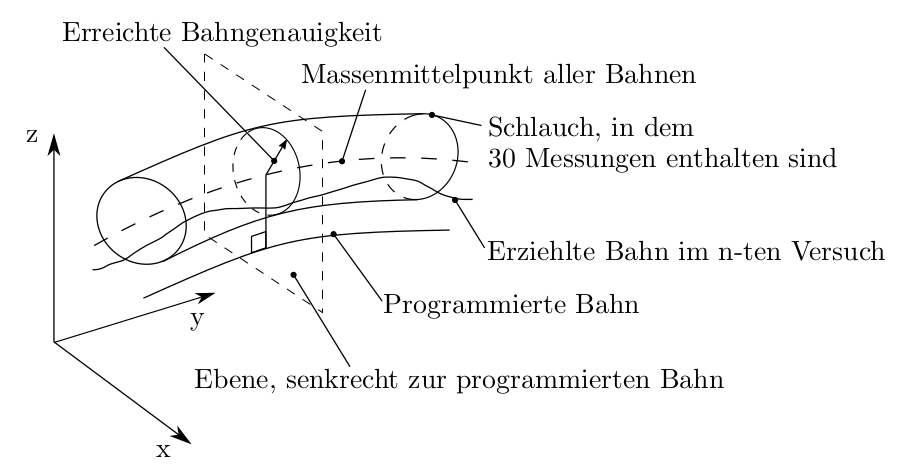
\includegraphics[width=0.9\textwidth]{images/stand_der_technik/bahngenauigkeit}
	\caption[Bahngenauigkeit]{Bahngenauigkeit \\Quelle: \cite[30]{pott_industrielle_2019}}
	\label{fig:bahngenauigkeit}
\end{figure}
\FloatBarrier

Bei einer großen Abweichung der Absolutgenauigkeit führt dies jedoch zu einem schlechten erreichen der Zielpose und dadurch auch zu einem schlechten Bahnverhalten wie in Abbildung \ref{fig:bahngenauigkeit} durch die erzielte Bahn im n-ten Versuch ersichtlich ist. Aus diesem Grund bieten viele Hersteller gegen einen Aufpreis absolutvermessene Industrieroboter an um diesen Genauigkeitsfehler zu kompensieren \cite[29\psq]{pott_industrielle_2019}. Wenn eine sehr hohe Wiederholgenauigkeit gewünscht ist kann auch mit Spezialrobotern eine Wiederholgenauigkeit von bis zu 1 \si{\micro}m erreicht werden \cite{noauthor_genauigkeit_nodate}.

\begin{figure}[htb]
	\centering
	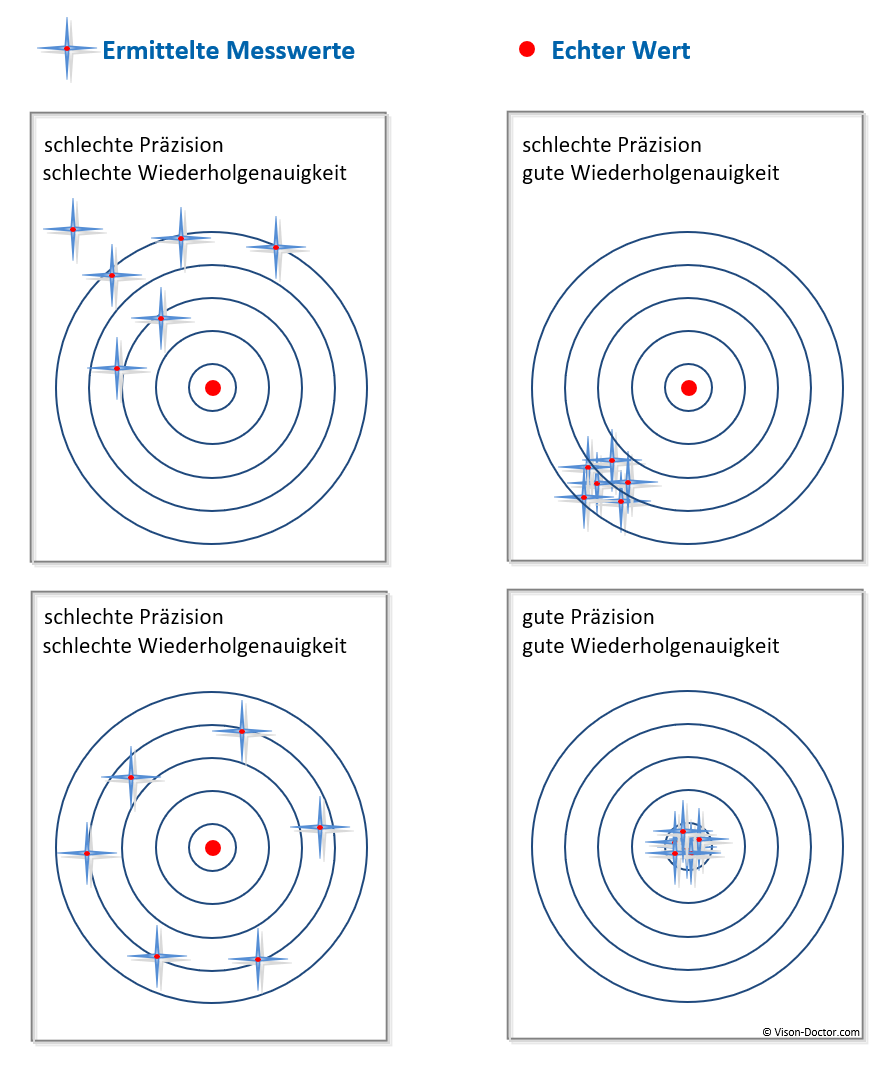
\includegraphics[width=0.57\textwidth]{images/stand_der_technik/wiederholgenauigkeit}
	\caption[Wiederholgenauigkeit]{Wiederholgenauigkeit \\Quelle: \cite{noauthor_prazision_nodate}}
	\label{fig:wiederholgenauigkeit}
\end{figure}
\FloatBarrier

Wie in Abbildung \ref{fig:wiederholgenauigkeit} zu sehen ist, kann daraus geschlossen werden, dass keine hohe Präzision durch eine schlechte Wiederholgenauigkeit möglich ist. Aus diesem Grund kann auch gesagt werden, dass die Wiederholgenauigkeit entscheidenter als die Absolutgenauigkeit zum erreichen der Zielposition ist, da umgekehrt nicht gesagt werden kann, dass eine hohe Präzision durch eine gute Wiederholgenauigkeit erreicht wird \cite{noauthor_genauigkeit_nodate}.


% S. 29 pott_industrielle_2019





% https://books.google.at/books?id=ajERH2hUuqYC&pg=RA4-PA2&lpg=RA4-PA2&dq=wiederholgenauigkeit+vs+%22absolutgenauigkeit%22+erkl%C3%A4rt&source=bl&ots=xG5j5lzFUK&sig=ACfU3U1u5fA3eDaQ6OjY5r5YH58DLxhdQg&hl=de&sa=X&ved=2ahUKEwizm-PP9uHpAhWJCOwKHdQgCS0Q6AEwCXoECAgQAQ#v=onepage&q=wiederholgenauigkeit%20vs%20%22absolutgenauigkeit%22%20erkl%C3%A4rt&f=false

% schönes bild & formel: https://www.vision-doctor.com/wiederholgenauigkeit.html
% https://www.fachwissen-technik.de/messtechnik/praezision-genauigkeit.html
% Die Stärke von Robotern ist also die Wiederhol- und weniger die Absolutgenauigkeit. (https://automationspraxis.industrie.de/robotik/hochgenaue-roboter/)
% Robotergenauigkeit ist, definiert die ISO 9283
% Die Wiederholgenauigkeit beschreibt, wie genau ein Robotersystem eine einmal angefahrene Position beim erneuten Anfahren erreicht. 
% Die Absolutgenauigkeit hingegen beschreibt, wie genau ein Robotersystem eine theoretisch programmierte Position in der Realität anfährt. Typischerweise sollten Robotersysteme standardmäßig auf 0,1 mm wiederhol- und auf 1 mm absolutgenau sein.
% Verschiedene Ursachen können dazu führen, dass ein Robotersystem ungenau arbeitet. Großen Einfluss haben hierbei die Getriebesteifigkeit unter Eigenlast und auch im Prozess, Justagefehler der Achsen, die Umgebungstemperatur und die thermische Ausdehnung durch die Motorwärme. Ganz simpel können auch Kollisionen die Genauigkeit reduzieren und einen Justagefehler verursachen, weil die Nullstellung der Winkelgeber in den Antrieben dabei verschoben wird. 
% oboter noch im Werk kalibriert, um Fertigungstoleranzen auszugleichen. Hinzu kommen jährliche Überprüfungen.
% Der wichtigste Vorteil eines ausreichend genauen Robotersystems ist die erwähnte Übereinstimmung zwischen theoretisch programmierter und tatsächlich erreichter Pose, weil dann das Nachteachen entfällt bzw. nur geringen Aufwand erfordert. 


% "Die Wiederholgenauigkeit beschreibt einfach ausgedrückt die Fähigkeit eines Roboters einen einmal geteachten Punkt immer wieder durch anfahren zu erreichen. Die ist bei den meisten IR sehr gut und liegt üblicherweise um 0,02 mm. Je nach Größe des IR.
% Die Absolutgenauigkeit ist die Fähigkeit bestimmte Punkte ausgehend vom Roboterkoordinatensystem zu erreichen ohne diese zu teachen. Hierbei stinken die meisten IR ab, das spiegelt sich bspw. in einem schlechten Bahnverhalten wieder, etc.
% oberallgeier hat natürlich recht! Die Absolutgenauigkeit hat Ihre Grenzen beim ca. dreifachen der Wiederholgenauigkeit.
%Die genaue Definition findest Du in der EN ISO 29283 (ehemals ISO 9283). Dort wird auch beschrieben, wie man die Genauigkeiten ermittelt." (https://www.roboternetz.de/community/threads/35643-absolutgenauigkeit)



% ----------------------

% S. 25 pott_industrielle_2019   kinematische Transformation (direkte & indirekte Transformation)
% cBei seriellen Robotern ist die direkte Kinema- tik stets eindeutig, während es für eine gewünschte Position des Endeffektors häufig mehr als eine Lösung gibt. Bei Knickarmrobotern kann es je nach Position bis zu acht mögliche Achsstellungen für eine vorgegebene Position des Endeffektors geben.``



% S. 54 - 56 pott_industrielle_2019

%\subsection{Bewegungsdynamik}
%\subsection{Steifigkeit}




% https://www.youtube.com/watch?v=wKiJaK-RDKI
% https://www.youtube.com/watch?v=GNrU2zviRpc



% https://de.wikipedia.org/wiki/Industrieroboter
% https://link.springer.com/chapter/10.1007%2F3-540-34823-9_27


% nach Kinematik unterschieden
% bestehen aus mehreren Gelenken
% serielle Roboter 95% & parallele 5% Roboter

% Arten & Vergleiche
% Genauigkeit
% Wie schnell können diese reagieren? (Zeitverhalten) je nach Roboterarm verschieden


\section{Arten von Teach Pendants}
% Arten von Handprogrammiergeräten
% Aufzählen
% Arten & Vergleiche
% Genauigkeit
% Wie funktioniert ein Teach Pendant
% Notaus stopp
% Welche Modies gibt es?
% Dead man's switch (https://de.wikipedia.org/wiki/Totmanneinrichtung)  (https://en.wikipedia.org/wiki/Dead_man%27s_switch)


\section{Arten von Zeitverhalten}
% Echtzeitverhalten
%    weiches & hartes Echtzeitverhalten
% Normales Zeitverhalten


\section{Sicherheitsanforderungen im Umgang mit Industrierobotern}


\section{ROS}
% Aufbauend auf dem Vergleich der Entwicklungsplattformen werden nun die für dieses Projekt am Besten geeigneten Werkzeuge vorgestellt.
% ROS 1 (LTS) vs ROS 2


\subsection{Architektur}


\subsection{Packages}


\subsection{Zukünftige Entwicklung}
% Community driven, ROS Foundation, ...


\subsection{Anbindungsmöglichkeiten/Interoperabilität}


\section{Simulations- und Testumgebungen}
% Gazebo, vRep, Coppelia Sim, ABB, ...


\section{Tiefensensoren}
% Arten und Vergleich (Vor- und Nachteile)
% Azure Kinect, ...
% Genauigkeit, Techniken, ...

\section{Gesten}
% Mögliche Gesten, Welche Gesten nicht


\section{Ergonomie}


\section{Sicherheit}
% https://de.wikipedia.org/wiki/Industrieroboter
% Maschinenrichtlinien
